\section{Sound and Light! (A Microphone and a Photocell)}
\label{lab_microphone_photocell}

%\makelabheader %(Space for student name, etc., defined in master.tex)

\bigskip

\begin{enumerate}[wide]

\item One place where field effect transistors are useful is in an electret microphone.  An electret is a material that holds a permanent polarization, something like the electric equivalent of a permanent magnet.  This material is mounted on a movable diaphragm that vibrates in response to sound, so that its vibration induces a small oscillating voltage in a nearby electrode.  A convenient way to detect this small voltage is to apply it to the gate of a field effect transistor.  Your microphone (the ``capsule,'' on the diagram) already has a transistor built into it.  Connecting the microphone to an external power source and resistor and removing the DC bias with a capacitor as shown produces an AC signal that's easy to measure.  How big is the resulting AC output when you whistle into the microphone?   (Note that the leads of your microphone are polarized; the negative terminal is the one that's visibly shorted to the outside of the capsule.)  
\begin{center}
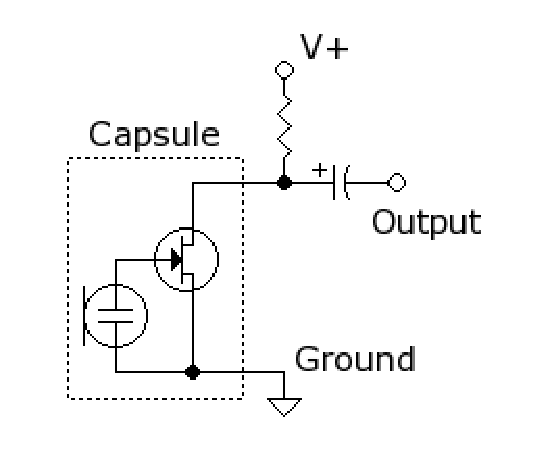
\includegraphics[width=2in]{microphone_photocell/microphone_schematic.eps}
\end{center}

\item As long as we're playing with detectors, your kits also include a photocell, or ``photoresistor.''  (It's the two-terminal thingy with a squiggly line on the top.) This is essentially a resistor made of cadmium sulfide, which is a semiconductor similar to silicon.  The resistivity of this material changes in response to light, as incident photons excite charge carriers across the band gap.  What is the resistance of this device in the ambient light of the room?  When you put your thumb over it?  Design and test a circuit that turns a current of 10~mA through an LED on and off  when you pass your hand over a photocell.
\begin{center}
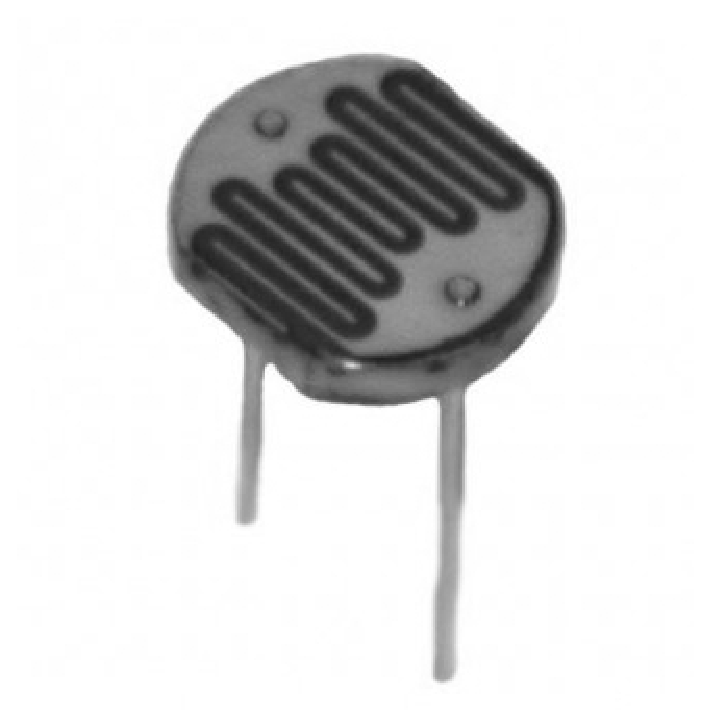
\includegraphics[width=1in]{microphone_photocell/photocell_bw.eps}
\end{center}


\end{enumerate}
